% this file is called up by thesis.tex
% content in this file will be fed into the main document

%: ----------------------- name of chapter  -------------------------
\chapter{Related Work} % top level followed by section, subsection


%: ----------------------- paths to graphics ------------------------

% change according to folder and file names
\ifpdf
    \graphicspath{{X/figures/PNG/}{X/figures/PDF/}{X/figures/}}
\else 
    \graphicspath{{X/figures/EPS/}{X/figures/}}
\fi

%: ----------------------- contents from here ------------------------

In this chapter, the basic principles of two critical components of any modern-day computer -- CPU and cache -- are described. An overview of the related to the thesis questions theory and publications is given. The chapter finishes with an evaluation of a number of existing benchmarks that can be used to test various aspects of the hardware.

\section{CPU}

The first x86 microprocessor Altair 8086 was created in 1978 \cite{gove2010multicore}. Since then the world has seen a number of improvements in performance of CPUs. The most measurable improvement has been gain in speed of processors that has come from increasing the clock speed (frequency at which a processor is running), and to a lesser extend through developing sophisticated in-build optimisation strategies.

Moreover, improvements in performance of processors were achieved by exploiting means of simultaneously performing multiple operations in a computer program -- instruction-level parallelism \cite{Hennessy2006}. Processors that use instruction-level parallelism are able to issue numerous instructions concurrently. In their pipelines, instructions are pre-fetched, split into sub-components and executed out-of-order \cite{schauer2008multicore}. The Pentium IV CPU released in 2000 was one of the last and the most powerful single-core processors \cite{Intel2000}. The “Prescott” and “Cedar Mill” cores from Pentium IV family featured as many as 31 stages in their pipelines, the longest in the history of mainstream computing \cite{Schmid2004}. However, there are certain factors that limit speed of systems that rely on this approach. Achieving satisfactory performance of instruction-level parallelism depends on efficiency of branch prediction performed by hardware or software. This is not trivial, which was proved as early as in 1991 \cite{Wall1991}. 

More recent advancements in the development of hardware for performing computations have mostly emphasised the importance of increasing the number of cores that are embedded on a single die\footnote{The word \textit{die} is used in a meaning of a computer chip throughout this document, unless stated otherwise.}, rather than experimenting with changing the clock rate or improving methods behind instruction-level parallelism. As a result, a new type of systems powered by a single processor that incorporates more that one central processing unit was developed. These cores are responsible for reading and executing instructions given to the CPU by programmes. Having additional cores on a silicon base improves performance and increases the upper bound of the amount of work that can be done by the processor by a factor of the total number of cores that the CPU obtains \cite{gove2010multicore}.

The motivation behind switching to multi-core systems resides in the fact that improving serial performance (performance of CPUs with one core) has become increasingly hard \cite{Jagtap2009}. One of the most commonly used methods of increasing speed of execution of commands in single-core processors is improving clock frequency by deeper pipelining. However, the advantage of utilising the deeper pipeline is reduced when the inserted Flip-Flop’s delay is comparable to the combinational logic delay. Such approach also increases cycles-per-instruction (CPI) and has a negatively impact on the overall system performance. Also, the number of logic gates in one pipeline stage determines the clock frequency. Reducing the segment size becomes hard on the smaller scale, creating a \textit{frequency wall}. In addition, the emergence of the \textit{power wall} means that the higher the clock speed, the more costly it is to remove heat, which applies limitations on the design and effectiveness of the system. 

To overcome the challenges in performance and power management, an innovative and different vision of the processor architecture and design had to be realised. The multi-core architecture is one of the most recent and promising technologies in the industry and starting from 2004 it has been dominating on the market of processors \cite{AMD2005,schauer2008multicore,Gepner2006}. A multi-core processor is a CPU that consists of multiple independent units that reside on the same processor chip, such structure is capable of executing instructions in a (not virtual) parallel fashion. Today multi-core processors may be found in all computer markets: server systems, desktop systems, mobile phones, and embedded systems. The popularity of this architecture is a true paradigm shift. A parallel computer is now a de facto machine for performing computation of all levels of complexity. \cite{Jagtap2009}

A shift to multi-core systems is beneficial for energy consumption since multi-core CPUs can allow both the clock frequency and supply voltage to be reduced when there is no need to perform heavy computation to avoid power overconsumption. Also, such systems are highly scalable since a single processor can be designed and a system could be built by linking together multiple processors. Furthermore, now multi-core processors also differ by a number of chips that they contain, i.e. one may buy a processor that consists of more than one independent CPU. With introduction of such new devices, the field of mass market computing entered a new era and with it a new need for performance analysis techniques and capabilities has risen.

\section{Cache}
\label{cacheLit}

A cache serves as a layer between a processor and main memory \cite{Langston2007}. A cache\footnote{The word \textit{cache} is used to refer to the memory cache throughout this document, unless stated otherwise.} is an essential component of any modern-day processor that by storing frequently-used data ensures that future requests for accessing that data are served faster. Cache can store both information that has been computed earlier and copies of data that is stored on other levels of memory hierarchy of the system. Data in caches is stored in basic units of cache storage, \textit{cache lines}, blocks of fixed size that may contain multiple bytes of memory. The minimum amount of information that can be read from a cache is one cache line, i.e. if one wants to read 1 byte of data stored in a cache of any level, the amount of data that is sent is still what is stored in one cache line (e.g. 64 bytes in the Xeon 5130). When caches are enabled, data and instructions go through the caches without the need for explicit software control. Additionally, utilisation of cache often creates a challenge of reducing the level of energy consumption \cite{Su1995}. Understanding the behavior of the cache is useful for optimising performance of both single- and multi-threaded software.

This project focuses on the Intel 64 architecture. Besides cache, this architecture also incorporates translation look aside buffers (TLBs)\footnote{\textit{Translation lookaside buffer} (TLB) is a new type of cache that is used to improve virtual address translation speed \cite{Arpaci-Dusseau2014}.}, and a store buffer for temporary on-chip (and external) storage of instructions and data \cite{Intel2014}. These technologies are only involved in virtual memory management, which is not a subject of this thesis. Figure \ref{xeon_cache_figure} shows the arrangement of caches, TLBs, and store buffers in Intel Pentium 4 and Intel Xeon CPUs. The cache normally consists of multiple levels \cite{Hennessy2006}. In modern microprocessors the primary cache is split into two caches of (normally) equal size -- one cache is used to store programme data, and the other one is used to hold microprocessor instructions. Some old microprocessors utilized ``unified'' primary cache, which was used to store both data and instructions in the same cache. In the case of Xeon processors, the Level 1 cache is divided into two sections. The Level 2 cache is shared between two chips in a dual-chip Xeon processor -- it is a unified data and instruction cache.

\begin{figure}[ht!]
\centering
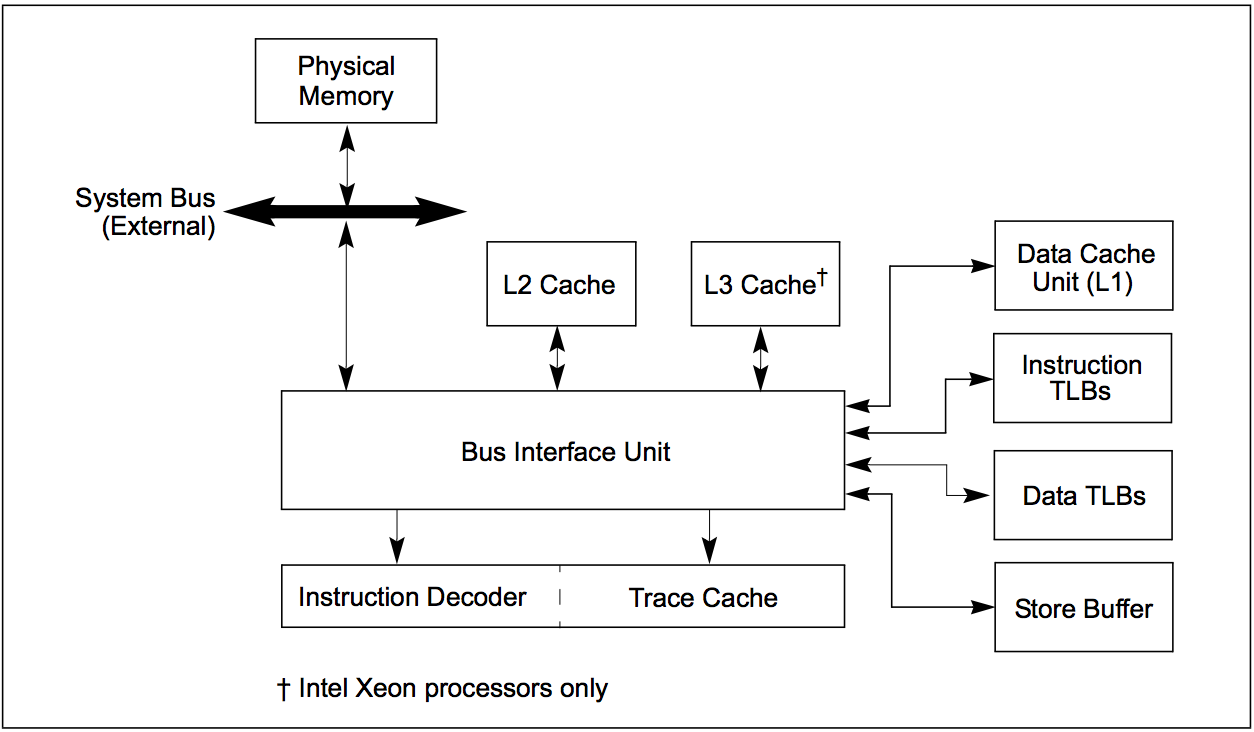
\includegraphics[width=145mm]{3/xeon_cache.png}
\caption{Cache Structure of the Pentium 4 and Intel Xeon Processors \cite{Intel2014}}
\label{xeon_cache_figure}
\end{figure}

Two other very important concepts are \textit{cache hits} and \textit{cache misses}. Cache hits occur when the cache can satisfy a request for the data required for further computation. If requested data cannot be found in the cache, of which the request was made, a cache miss occurs. Cache hits are a desired property of a computational system because they improve overall performance by reducing overhead caused by accessing data from bigger and slower levels of the memory hierarchy (e.g. RAM, a hard disk); system architects try to reduce the number of cache misses. Essentially, the larger the amount of data that can be provided directly from the cache, the greater the speed. The cache miss ratio is one of the ways to measure efficiency of cache usage; the lower the cache miss ratio, the faster the system is \cite{Chen2007}. Also, it is important to know that a \textit{cache line fill} happens when the CPU sees that a quantum of data, that is being read from memory, can be stored in a cache; the memory controller writes an entire cache line into the appropriate level(-s) of cache \cite{Intel2014}.

Studies indicate that fast cache-to-cache communication is crucial for achieving the best performance and scalability of multi-threaded programmes \cite{Molka2009,Lo2013,Zhang2010}. However, with increases in the clock rate, the system starts to suffer from the high level of cache miss ratio: caches are used more intensly. Heavy usage of processor hardware support (utilising larger caches and branch tables) and a bigger level of awareness on memory performance have helped processor designers manage cache misses and branches \cite{Jagtap2009}.

A term \textit{bus sniffing} is commonly used to describe a technique that is employed to support \textit{cache coherence}, i.e. the consistency of data stored in different levels of cache \cite{Hennessy2006}. Each controller of cache monitors instructions that may invalidate a cache line in the cache. They ensure that the same memory location is not loaded into more than one cache and if a quantum of data is requested, only one value is returned from all levels of memory \cite{Neupane2004}.

A fundamental decision in cache design is whether each piece of data can be stored in a cache once (in any cache line), or in only some of the lines \cite{Ostrovsky2010}. It is called \textit{cache associativity}. One may define three distinct types of cache associativity based on the way information is stored in the cache \cite{Hennessy2006}:

\begin{description}
  \item[Direct mapped cache] Each quantum of data can be saved in only a single cache line. It makes a cache block of data easy to find, but cache loses in flexibility of allocation of data.
  \item[N-way set associative cache] Every piece of data can be stored in one of N lines in the cache. For example, in a 8-way set associative cache, each quantum of data can saved in 8 different lines of cache. The index must be implemented to support locating data within the set.
  \item[Fully associative cache] Each quantum of information can be saved in any cache line; one may say that the cache works as a simple hash-table. Every tag associated with a quantum of data in the cache must be compared when looking for a block of data in the cache, but placement of data is simplified.
\end{description}

Figure \ref{cache_diagram} shows an example of a direct mapped cache and its interaction with blocks of data in main memory. Each block in main memory is associated with exactly one block in a cache.

\begin{figure}[ht!]
\centering
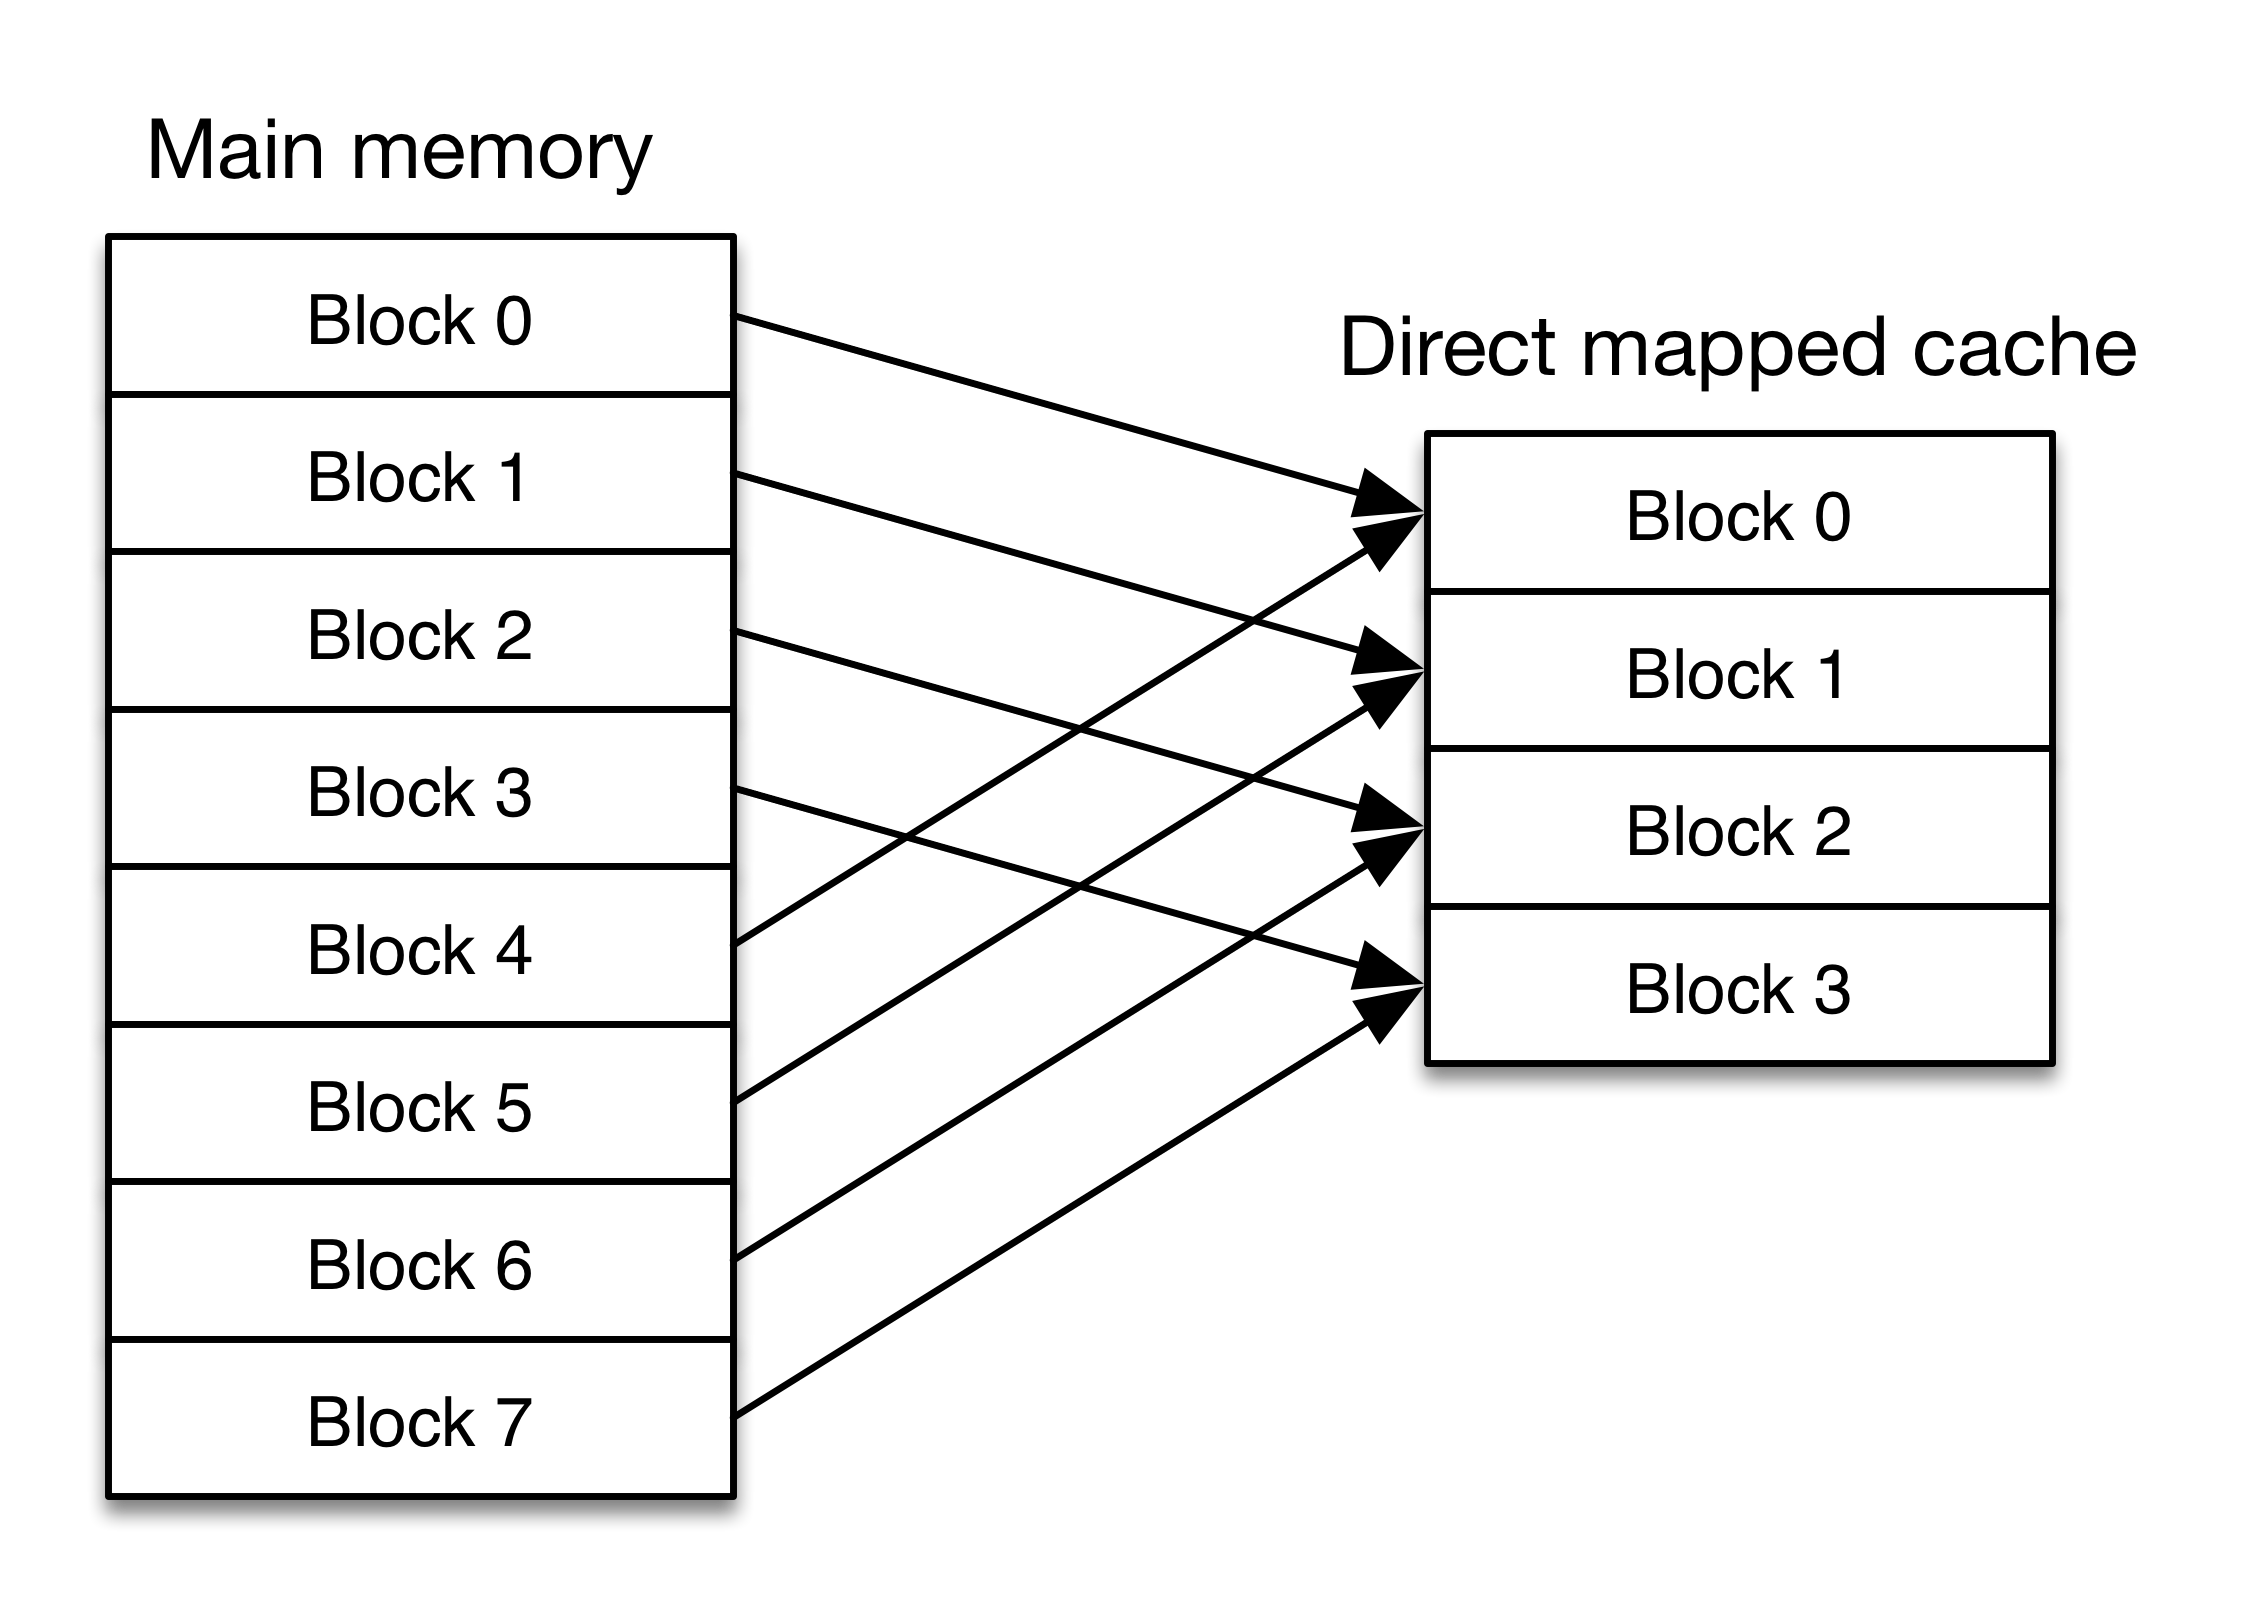
\includegraphics[width=100mm]{3/cache_diagram.png}
\caption{An example of a direct mapped cache}
\label{cache_diagram}
\end{figure}

Then, there are two main methods of caching (organising access to caches) available \cite{Intel2014}:

\begin{description}
  \item[Write-back (WB)] Both operations of writing and reading data to and from main memory are stored in caches. Data being cached is written only to the cache. The cached data is used to update main memory. This type of caching decreases bus traffic by eliminating many unnecessary writes to main memory. Processors used in this research have Write-back caches.
  \item[Write-through (WT)] Both operations of writing and reading data to and from main memory are also stored in caches. Data being cached is written both to the cache and to the main memory. When writing through to main memory, unused cache lines are not cleaned (indicate that it was unchanged since it was read from main memory), and valid cache lines are either filled (references memory in main memory when a word is not found in cache) or invalidated (marked as having incoherent copy of data in main memory). A write operation is not considered complete until the write to main memory is finished.
\end{description}

Finally, performance of processors is often impacted by implicit and explicit caching \cite{Intel2014}. \textit{Implicit caching} occurs when a piece of memory is marked as \textit{potentially cacheable}, although the element may never have been accessed. Implicit caching occurs in recent processor families due to data prefetching, branch prediction\footnote{\textit{Branch prediction}: when a CPU attempts to guess in which way a logical branch (e.g. if-then-else statement) will be executed before it can be known with certainty.}, and TLB miss handling. \textit{Explicit caching} is observed due to overuse of prefetch instructions (e.g. \textit{PREFETCHh} instruction, which was introduced in the Pentium III processor family). These instructions give ``hints" that a quantum of data will be used soon and should be cached as soon as possible. The explicit caching can lead to resource conflicts, which decrease the performance of an application. These events are difficult to handle on the software level and should be eliminated on the OS level.

\subsection{Cache Affinity}

One of the most commonly used metrics for measuring performance of multi-threaded systems is cache affinity \cite{Torrellas1995,Squillante1993,Vaswani1991}. Cache affinity is described as the amount of process's data or instructions stored inside of the cache. Affinity can be both high and low, depending on how much state has been accumulated. Speed of multi-threaded programmes is affected by the ability of processor cores to get access of required data by traveling through as few levels of cache and memory as possible \cite{Kazempour2008}. Cache affinity is often exploited by schedulers (algorithms that load-balance workload on processors) by rescheduling processes to run on a recently used processor.

Cache affinity has a direct impact on the level of cache misses in the system. The cache miss penalty to main memory, which costs hundreds of CPU cycles, and complexity of hardware that needs to be built, often reduce benefits that can be achieved from implementing instruction-level parallelism \cite{McKee2004}. Reduction of cache misses is beneficial for improving performance as well, as was shown in the project conducted by the author in the University of St Andrews \cite{Bazilinskyy2013}.

\subsection{Cache Latency and Throughput}

\textit{Cache latency} is the time taken to access a block of data in a cache. \textit{Cache throughput} is the amount of data that can be accessed in a unit of time. It is desirable to read as much data as quickly as possible, hence the lower the latency and the higher the throughput, the better.

CPUs often contain data \textit{prefetchers}, which transfer information into caches heuristically, i.e. they predict which data will also be accessed in the future and store it in the cache to be ready when required \cite{HasinaKhatoonShahidHafeezMirza2013}. By using the data prefetchers, one may reduce the amount of time that the CPU has to wait for the data to be fetched, i.e. data does not have to travel all the way from the main memory, but only from the faster cache. The Xeon processors used in the study utilise hardware data prefetchers \cite{Intel2009b}.

Applications often use data that is stored closely to what has been referenced recently, it is known as \textit{data locality}. There are two kinds of locality: 1) \textit{Temporal locality}: where there is a relatively big chance that a recently used quantum of data is likely to be used again in the near future; 2) \textit{Spatial locality}: pieces of data with nearby addresses are often referenced close together in time \cite{Denning2005}. Data Locality of information stored in the cache has a particularly large effect on the speed of multi-threaded applications \cite{ChenDing,Schneider2006}.

Data prefetchers use the principles of data locality and operate by analysing patterns in the access of data during the execution of programmes. Therefore, latency and throughput of accessing data depend on whether the prefetchers have been successful at comprehending the pattern of data usage and whether they have fetched the right piece of information into the caches. \cite[p.~811]{ward1990computation}

Cache latency and throughput affect both unichip and multichip systems. Benefits that can be received through reducing cache latency and increasing cache throughput differ across various multi-core architectures, i.e. multi-core uniprocessors and multi-core multiprocessors. The topic of the impact of the cache on speed of software has been discussed in the scientific community for more than two decades now; some examples of published results may be found in \cite{torrellas1995evaluating, Chen2007,VineethMekkatAnupHoleyPen-ChungYew2013}. The paper \cite{torrellas1995evaluating} proposed an algorithm for affinity-aware scheduling of threads that reduces the number of cache misses by up to 36\%; however, it was written in 1995 and the results cannot be considered as applicable to the modern-day computer architecture. The authors of \cite{Chen2007} merely discuss already built solutions that were developed in 1990s, and \cite{VineethMekkatAnupHoleyPen-ChungYew2013} focuses only on the shared last-level cache (LLC). Considerably fewer resources discuss the effect of cache on multi-core than on classic single-CPU architectures.

To summarize, the speed of multi-threaded programmes depends on a number of processes, as well as attributes associated with caches. This section has discussed a number of them: cache interference and cache miss ratio, the way caching is handled, and cache associativity. The context survey revealed that the impact of cache on data-sharing in multi-threaded environments is not covered extensively in published research. The motivation for this project came after realising that modern Linux kernels do not take the impact of the cache into account when scheduling of threads takes place in multi-core environments \cite{Bovet:2005:ULK:1077084,Aas2005}. Therefore, creation of a model of inter-thread communication in multi-core systems is investigated. The theoretical background offered by the model is tested by conducting a number of experiments on real hardware that form two distinct multi-core systems. A taxonomy of inter-thread communication is presented to support the model.

\section{Benchmarks for Testing Performance of Cache in Multi-Core Systems}
\label{sec:benchmarks}

A number of existing benchmarking suites were evaluated to understand if existing solutions could be utilised for answering the research questions. Providing a standardised set of tools for measuring and comparing performance of different parts of the system is currently a widely-discussed topic. Standardisation organisations\footnote{\url{http://www.spec.org/}} and conferences focused on the topic\footnote{\url{http://icpe2014.ipd.kit.edu/}}, that are meant to help software developers and hardware vendors, are emerging.

System- and component-level benchmarking tools were analysed. Namely: lmbench\footnote{\url{http://www.bitmover.com/lmbench/}}, Intel's VTune\footnote{\url{https://software.intel.com/en-us/intel-vtune-amplifier-xe}}, Valgrind\footnote{\url{http://valgrind.org/}}, and CPU2000\footnote{\url{https://www.spec.org/cpu2000/}}. VTune is a popular solution that is commonly used for fine-tuning high performance software that relies on hardware from Intel; it is not applicable to this study because of limited support for underlying libraries in the laboratory settings and lack of documentation on measuring latency and throughput of different layers of memory. It was found that Valgrind does not perform simulation on physical hardware, but, rather, through virtualisation, in this instance it cannot guarantee accuracy of results achieved from experiments. In addition, CPU2000 is an outdated product that is not supported by its developers and hence it offers little value to the scientific community. The tool lmbench is an open-source solution that was developed in early 1990s. Despite the lack of extensive documentation, it was possible to confirm that it is capable of checking latency of accessing cache.

% ---------------------------------------------------------------------------
%: ----------------------- end of thesis sub-document ------------------------
% ---------------------------------------------------------------------------

